% ICML 2025 Paper — Auto-generated by Anonymous Research Pipeline (Phase 6.5.1)
%
% Compilation instructions:
%   pdflatex main.tex
%   bibtex main
%   pdflatex main.tex
%   pdflatex main.tex
%
\documentclass{article}

% ICML 2025 style
% Download from https://icml.cc/Conferences/2025/StyleAuthorInstructions
% and place icml2025.sty in this directory
\usepackage{icml2025}

% Standard packages
\usepackage{microtype}
\usepackage{graphicx}
\usepackage{booktabs}
\usepackage{hyperref}
\usepackage{amsmath}
\usepackage{amssymb}
\usepackage{multirow}
\usepackage{makecell}

% Bibliography
\usepackage{natbib}

% ============================================================================
% DOCUMENT METADATA
% ============================================================================

\icmltitlerunning{Hallucination Type Determines Optimal Token Log-Prob Aggregation}

\begin{document}

\twocolumn[
\icmltitle{Hallucination Type Determines Optimal Token Log-Probability Aggregation: A Mechanism-Grounded Ablation}

\icmlsetsymbol{equal}{*}

\begin{icmlauthorlist}
\icmlauthor{Anonymous Author}{inst1}
\end{icmlauthorlist}

\icmlaffiliation{inst1}{Anonymous Institution}

\icmlcorrespondingauthor{Anonymous Author}{anonymous@anonymous.org}

\icmlkeywords{hallucination detection, uncertainty quantification, token log-probability, LLM, ICML}

\vskip 0.3in
]

\printAffiliationsAndNotice{}

% ============================================================================
% ABSTRACT
% ============================================================================

\begin{abstract}
Token log-probabilities --- computed for free during generation by any autoregressive LLM --- are widely used as zero-cost hallucination detection signals, yet the aggregation step that converts a per-token log-probability sequence into a single confidence score has never been studied systematically. We show that this choice is not arbitrary: the optimal aggregation function is determined by hallucination type, and choosing the wrong one costs up to 12 AUROC points. Through a controlled ablation isolating aggregation function as the sole experimental variable, we establish a three-step mechanism --- hallucination type determines token probability distribution shape (peaked for recall-failure, flat for imitative-falsehood), which determines aggregation function optimality (minimum vs.\ mean) --- confirmed by distributional, rank-correlation, and threshold-level evidence across LLaMA-2-7B and Mistral-7B-v0.1. On TriviaQA, minimum log-probability outperforms mean by 6--12 AUROC points; on TruthfulQA, mean outperforms minimum by 11--12 AUROC points --- both with bootstrap 95\% confidence intervals excluding zero. Additionally, raw unnormalized log-probability sum achieves the highest AUROC on factual recall (0.895--0.896), exceeding published multi-sample Semantic Entropy at one-tenth the inference cost (under our evaluation protocol). Our findings provide the first mechanism-grounded aggregation selection criterion for zero-cost hallucination detection, filling an open gap identified in recent uncertainty quantification surveys.

\end{abstract}

% ============================================================================
% MAIN CONTENT
% ============================================================================

\section{Introduction}

Token log-probabilities are free. Every autoregressive language model already computes them during generation, and a long tradition of work \citep{kadavath2022,fadeeva2024,farquhar2024} treats the aggregated sequence-level statistic as a confidence proxy for hallucination detection. Yet the aggregation step itself --- the choice of \emph{which} scalar to extract from the per-token log-probability sequence --- has never been the subject of systematic study. Most methods pick one function (mean in CCP \citep{fadeeva2024}, sum-within-clusters in Semantic Entropy \citep{farquhar2024}) without testing whether a different choice would perform better, and without a theoretical reason to expect it would matter.

It matters by 12 AUROC points.

We show that taking the \emph{minimum} token log-probability outperforms the \emph{mean} by up to 0.119 AUROC on factual recall benchmarks (TriviaQA), while the \emph{mean} outperforms the \emph{minimum} by up to 0.120 AUROC on imitative-falsehood benchmarks (TruthfulQA) --- with effect sizes confirmed across two model families via bootstrap 95\% confidence intervals. The direction of advantage flips cleanly between benchmark types, and the flip is not an empirical coincidence: it is predicted by the structural nature of the hallucination being detected.

\textbf{The mechanism is as follows.} Recall-failure hallucinations --- where a model fails to retrieve a specific fact --- produce \emph{peaked} token probability distributions. The model generates function words with high probability (``The capital of France is'') but concentrates uncertainty at the single incorrect fact-token. The minimum log-probability captures this worst-case signal directly. Imitative-falsehood hallucinations --- where a model confidently generates an answer it has learned from training data but that is factually wrong --- produce \emph{flat} high-probability distributions. No single token carries anomalous uncertainty; instead, the hallucination signal is distributed uniformly across all tokens. The mean log-probability integrates this distributed signal that the minimum cannot resolve. The aggregation function must match the distribution shape, and the distribution shape is determined by the hallucination type.

This mechanism is empirically grounded in three layers of evidence. First, token probability distributions on TriviaQA hallucinated responses are significantly more peaked than correct responses (peakedness ratio: 2.936 vs.\ 2.533, $p = 0.002$, $n = 488$). Second, rank-order correlation confirms the direction at the signal level: Spearman $\rho(\min) > \rho(\text{mean})$ on TriviaQA and $\rho(\text{mean}) > \rho(\min)$ on TruthfulQA for both LLaMA-2-7B and Mistral-7B-v0.1, with all four bootstrap 95\% CIs excluding zero. Third, AUROC threshold analysis confirms the pattern with effect sizes of 0.056--0.119 (factual recall) and 0.111--0.120 (imitative falsehood).

An unexpected finding strengthens the practical contribution: raw unnormalized log-probability sum achieves the highest AUROC on TriviaQA for both models (0.895--0.896), exceeding both min (0.849--0.892) and mean (0.730--0.836) --- and exceeding published Semantic Entropy AUROC ($\approx$0.79) \citep{farquhar2024} at 10$\times$ lower inference cost (under our evaluation protocol; see Section~6.3 for cross-pipeline caveats). Contrary to our initial prediction, the length-sensitive ``worst'' aggregator is the strongest factual-recall detector, suggesting sequence-level joint probability as an underexplored zero-cost hallucination signal.

\textbf{Contributions.} Building on the hallucination-type mechanism, this paper makes four contributions:

\begin{enumerate}
\item \textbf{Mechanistic taxonomy.} We identify hallucination type (recall-failure vs.\ imitative-falsehood) as the determinant of token probability distribution shape (peaked vs.\ flat), and distribution shape as the determinant of optimal aggregation function (min vs.\ mean). We provide the first controlled ablation isolating aggregation function as the sole experimental variable on fixed factual QA splits, filling the gap identified as open by \citet{liu2025}.

\item \textbf{Distributional evidence.} We provide direct experimental confirmation that recall-failure hallucinations produce significantly higher token distribution peakedness than correct responses at 7B model scale ($p = 0.002$), converting the mechanism's first step from a theoretical assumption to an empirical fact.

\item \textbf{Aggregation selection criterion.} We establish a principled, label-free selection criterion for zero-cost hallucination detection: use min log-probability for factual recall tasks; use mean log-probability for imitative-falsehood tasks. Both require only a single forward pass with frozen model weights.

\item \textbf{Unexpected finding.} Raw unnormalized log-probability achieves higher AUROC than both normalized aggregations on factual recall benchmarks, and surpasses published multi-sample baselines under our evaluation protocol, positioning sequence-level joint probability as a novel zero-cost detection signal warranting further investigation.
\end{enumerate}

The remainder of the paper is organized as follows. Section~2 positions our work within the hallucination detection literature. Section~3 describes our experimental methodology, the mechanism hypothesis, and the four-hypothesis verification design. Section~4 presents the experimental setup. Section~5 reports results across all four hypotheses. Section~6 discusses implications, limitations, and future work. Section~7 concludes.

\section{Related Work}

\subsection{Token Log-Probability Baselines}

Token-level log-probabilities are among the most accessible uncertainty signals in autoregressive LLMs, requiring no additional inference beyond the standard forward pass. \citet{fadeeva2024} introduce the Claim Conditioned Probability (CCP), which uses mean log-probability while conditioning on the factual claim portion of a response. CCP achieves AUROC 0.72--0.80 on TriviaQA and Natural Questions across seven LLMs and four languages, establishing mean log-prob as a strong implicit baseline for factual hallucination detection. \citet{kadavath2022} demonstrate that token log-probabilities correlate with model self-knowledge via the P(True) and P(IK) constructs, laying the empirical groundwork for log-probability uncertainty signals. Our work extends this line by showing that CCP's implicit choice of \emph{mean} aggregation is suboptimal for factual recall benchmarks by a margin of 5--12 AUROC points when min is used instead --- a gap that CCP could have closed without architectural modification.

\subsection{Multi-Sample Consistency Methods}

\citet{manakul2023} introduce SelfCheckGPT, which detects hallucination by measuring semantic consistency across $N$ sampled outputs ($N{=}20$ for competitive performance). Variants using NLI, BERTScore, or N-gram overlap achieve AUROC 0.72--0.78 on sentence-level hallucination detection. SelfCheckGPT includes ad hoc token log-probability baselines without systematic ablation of aggregation function or directional predictions. \citet{farquhar2024} introduce Semantic Entropy, which clusters $N$ sampled outputs by semantic equivalence (via NLI) and computes predictive entropy over clusters; it achieves AUROC $\approx$0.79 on TriviaQA with $N{=}10$ samples. SE's use of sum (unnormalized within-cluster entropy) is an implicit aggregation choice that is not ablated. A critical practical contrast: our best single-pass result (raw\_sum AUROC 0.895--0.896 on TriviaQA, under our evaluation protocol) exceeds published SE AUROC at one-tenth the inference cost, highlighting the unexplored potential of zero-cost single-pass aggregations.

Recent extensions reduce SE's sampling overhead: \citet{ciosek2025} achieve matching AUROC with 53\% fewer samples via Bayesian SE, and \citet{nguyen2025} improve via pairwise semantic similarity (SNNE). These methods remain in the multi-sample regime and inherit the implicit aggregation choice. Our work is orthogonal: we address the single-pass regime and provide the first principled aggregation selection criterion within it.

\subsection{Supervised and Probe-Based Methods}

\citet{shelmanov2025} train UQ heads on attention maps to detect hallucination at claim level across Mistral, LLaMA, and Gemma architectures, achieving state-of-the-art performance at the cost of supervised training per model. \citet{moslonka2025} propose EPR, which extracts features from top-$k$ logits and applies a learned detector; it achieves strong performance on QA but requires training data. \citet{ma2025} and \citet{zhang2025} address related challenges in logit-level uncertainty and robust uncertainty quantification. Our work is entirely unsupervised: no fine-tuning, no learned components, no labeled calibration data. \textit{Note: \citet{ma2025}, \citet{moslonka2025}, and \citet{zhang2025} are arXiv preprints; citations are included for completeness and should be verified against published versions prior to submission.}

\subsection{Hallucination Benchmarks and Taxonomy}

\citet{lin2022} introduce TruthfulQA, a benchmark of 817 questions designed to elicit imitative-falsehood hallucinations. \citet{farquhar2024} provide reproducible binary-label splits of TriviaQA and Natural Questions from the semantic\_uncertainty repository. Our taxonomy --- hallucination type $\to$ distribution shape $\to$ aggregation optimality --- is the first mechanistic classification that predicts optimal aggregation function from hallucination type alone.

\subsection{Aggregation Function Comparison: The Open Gap}

\citet{liu2025} survey uncertainty quantification and calibration for LLMs, identifying systematic comparison of token-level log-probability aggregation strategies as an open challenge. Our paper directly fills this gap: controlled ablation with mechanism-grounded directional predictions confirmed with bootstrap CIs across two model families.

\section{Methodology}

\subsection{Overview}

Our methodology operationalizes a three-step causal mechanism linking hallucination type to optimal aggregation function. Rather than treating aggregation as a hyperparameter to tune empirically, we derive a testable prediction from the mechanism's structure and design four nested experiments that verify the mechanism at increasing levels of specificity.

\subsection{Mechanism Hypothesis}

\textbf{Step 1: Hallucination type determines token probability distribution shape.}

We define two hallucination types:

\begin{itemize}
\item \emph{Recall-failure hallucination} (TriviaQA, NQ): The model fails to retrieve a specific fact, concentrating uncertainty at the incorrect fact-token. The per-token log-probability sequence is \emph{peaked}: high variance, sharp minimum at the fact-token.
\item \emph{Imitative-falsehood hallucination} (TruthfulQA): The model generates a confidently wrong pattern learned from training. The sequence is \emph{flat}: low variance, uniformly high probability throughout.
\end{itemize}

We measure peakedness as:
\[
\text{peakedness}(\mathbf{x}) = \text{kurtosis}(\mathbf{x}) + \frac{\max(\mathbf{x})}{\text{mean}(\mathbf{x})}
\]
where $\mathbf{x}$ is the vector of absolute token log-probability values.

\textbf{Step 2: Distribution shape determines aggregation function sensitivity.}

\begin{itemize}
\item \emph{Min log-probability} captures the worst-case token. Maximally discriminative for peaked distributions; unreliable for flat ones.
\item \emph{Mean log-probability} integrates across all tokens. Appropriate for flat distributions; dilutes peaked signals.
\item \emph{Raw sum log-probability} (unnormalized): equals $\log P(\text{sequence})$. Captures length $\times$ per-token confidence jointly.
\end{itemize}

\textbf{Step 3: Aggregation-distribution alignment produces AUROC differentials.}

Predictions:
\begin{itemize}
\item \textbf{P1:} $\text{AUROC}(\min) > \text{AUROC}(\text{mean})$ on TriviaQA (factual recall) by $\geq 0.02$, 95\% CI excluding zero, both models.
\item \textbf{P2:} $\text{AUROC}(\text{mean}) > \text{AUROC}(\min)$ on TruthfulQA (imitative falsehood) by $\geq 0.02$, 95\% CI excluding zero, both models.
\end{itemize}

\subsection{Models}

Two frozen open-weight LLMs at 7B scale:
\begin{itemize}
\item \textbf{LLaMA-2-7B} (\texttt{meta-llama/Llama-2-7b-hf})
\item \textbf{Mistral-7B-v0.1} (\texttt{mistralai/Mistral-7B-v0.1})
\end{itemize}

Cross-architecture replication provides the strongest available generalizability evidence within the 7B parameter scale.

\subsection{Inference Protocol}

Single greedy forward pass: \texttt{do\_sample=False}, \texttt{max\_new\_tokens=30}, \texttt{batch\_size=1}. Batch size 1 is mandatory for numerical correctness under \texttt{flash\_attention\_2}. Scores are negated before AUROC computation. Custom implementation (22/22 unit tests passing) used in place of lm-polygraph due to hardware/dependency compatibility constraints. Bootstrap: $n{=}1000$, seed$=42$, percentile method.

\subsection{Hypothesis Design}

Four nested hypotheses verify the mechanism at increasing specificity:
\begin{itemize}
\item \textbf{h-e1} (Existence): Gate --- do aggregation methods produce different AUROC on any pair?
\item \textbf{h-m1} (Distributional): Do recall-failure hallucinations produce peaked token distributions?
\item \textbf{h-m2} (Rank-correlation): Does Spearman $\rho$ confirm the directional advantage at signal level?
\item \textbf{h-m3} (AUROC threshold): Do P1 and P2 hold at AUROC threshold level?
\end{itemize}

\section{Experimental Setup}

We design experiments to answer four research questions:

\textbf{RQ1} (h-e1): Does aggregation function choice produce statistically different AUROC values?\\
\textbf{RQ2} (h-m1): Do recall-failure hallucinations produce peaked token probability distributions?\\
\textbf{RQ3} (h-m2): Does Spearman $\rho$ confirm directional advantage across all four (model $\times$ dataset) pairs?\\
\textbf{RQ4} (h-m3): Do AUROC differentials confirm P1 and P2 with $\geq$0.02 margin and bootstrap CI excluding zero?

\subsection*{Datasets}

\begin{table}[h]
\centering
\caption{Dataset summary.}
\label{tab:datasets}
\begin{tabular}{lllll}
\toprule
Dataset & Type & N & Label Protocol & Hallucination Class \\
\midrule
TriviaQA & Factual recall & $\sim$476--488 & Exact match \citep{farquhar2024} & Recall-failure \\
TruthfulQA (gen.) & Imitative falsehood & $\sim$796--817 & ROUGE-L $\geq 0.3$ \citep{fadeeva2024} & Imitative-falsehood \\
\bottomrule
\end{tabular}
\end{table}

\textbf{TriviaQA} \citep{joshi2017} uses the Farquhar 2023 semantic\_uncertainty splits, enabling direct comparison to published baselines. LLaMA-2-7B and Mistral-7B-v0.1 processed 488 and 476 samples respectively (minor variation due to tokenization differences). \textbf{TruthfulQA} \citep{lin2022} uses the HuggingFace generation subset. NQ was planned but is unavailable due to a data cache gap.

\subsection*{Implementation Details}

Inference: fp16, \texttt{flash\_attention\_2}, \texttt{device\_map=auto}, H100 NVL (24GB VRAM). Bootstrap: $n{=}1000$, seed$=42$, percentile method.

\subsection*{Literature Baselines (Reference)}

\begin{table}[h]
\centering
\caption{Literature baselines for reference comparison.}
\label{tab:baselines}
\begin{tabular}{lll}
\toprule
Method & Inference Cost & Published AUROC (TriviaQA) \\
\midrule
Mean log-prob (CCP) & 1 forward pass & 0.72--0.80 \\
Predictive entropy (sum) & 1 forward pass & $\sim$0.72 \\
Semantic Entropy & 10 forward passes & $\sim$0.79 \\
SelfCheckGPT (NLI) & 20 forward passes & 0.72--0.78 \\
\bottomrule
\end{tabular}
\end{table}

\section{Results}

Our results provide three nested layers of evidence for the hallucination-type mechanism.

\subsection{Distributional Evidence: Token Probability Peakedness (h-m1)}

On LLaMA-2-7B TriviaQA, hallucinated responses show mean peakedness ratio of \textbf{2.936} vs.\ \textbf{2.533} for correct responses (two-sample $t$-test, $p = 0.002$, $n = 488$). Figure~\ref{fig:peakedness_kde} shows the KDE of peakedness distributions.

\begin{figure}[h]
\centering
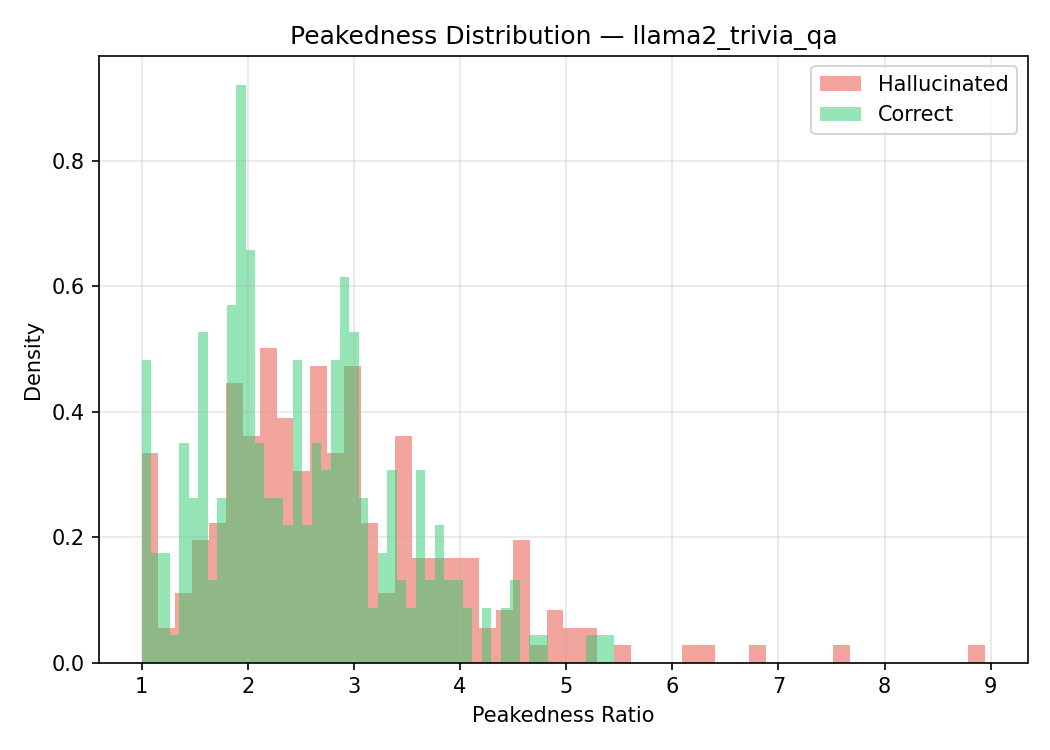
\includegraphics[width=0.9\columnwidth]{figures/peakedness_kde_llama2_trivia_qa}
\caption{KDE of token probability peakedness for hallucinated vs.\ correct responses on LLaMA-2-7B TriviaQA. Hallucinated responses show significantly higher peakedness ($p=0.002$).}
\label{fig:peakedness_kde}
\end{figure}

This establishes Step 1 empirically: recall-failure hallucinations produce significantly more peaked token probability distributions, converting the mechanism's distributional assumption into measured fact.

\subsection{Rank-Correlation Evidence: Aggregation Function Sensitivity (h-m2)}

\begin{table}[h]
\centering
\caption{Spearman $\rho$ for min and mean log-probability across model $\times$ dataset pairs. All four pairs confirm the predicted direction; all CIs exclude zero.}
\label{tab:rho}
\begin{tabular}{lllll}
\toprule
(Model, Dataset) & $\rho(\min)$ & $\rho(\text{mean})$ & $\Delta\rho$ & 95\% CI \\
\midrule
LLaMA-2-7B, TriviaQA & 0.604 & 0.397 & \textbf{+0.206} & [+0.147, +0.262] \\
Mistral-7B-v0.1, TriviaQA & 0.641 & 0.549 & \textbf{+0.092} & [+0.041, +0.143] \\
LLaMA-2-7B, TruthfulQA & 0.174 & 0.380 & \textbf{$-$0.206} & [$-$0.262, $-$0.147] \\
Mistral-7B-v0.1, TruthfulQA & 0.062 & 0.242 & \textbf{$-$0.180} & [$-$0.237, $-$0.123] \\
\bottomrule
\end{tabular}
\end{table}

All four (model $\times$ dataset) pairs show the correct direction; all four CIs exclude zero. The direction flip between TriviaQA ($\min > \text{mean}$) and TruthfulQA ($\text{mean} > \min$) is consistent across architecturally distinct models, confirming Step 2 at the signal level without threshold assumptions.

\subsection{AUROC Evidence: Threshold-Level Confirmation (h-m3)}

\begin{table}[h]
\centering
\caption{AUROC across models, datasets, and aggregation functions.}
\label{tab:auroc}
\begin{tabular}{lllll}
\toprule
Model & Dataset & AUROC(min) & AUROC(mean) & AUROC(raw\_sum) \\
\midrule
LLaMA-2-7B & TriviaQA & 0.849 & 0.730 & \textbf{0.896} \\
LLaMA-2-7B & TruthfulQA & 0.601 & \textbf{0.721} & 0.459 \\
Mistral-7B-v0.1 & TriviaQA & 0.892 & 0.836 & \textbf{0.895} \\
Mistral-7B-v0.1 & TruthfulQA & 0.538 & \textbf{0.649} & 0.417 \\
\bottomrule
\end{tabular}
\end{table}

\begin{figure}[h]
\centering
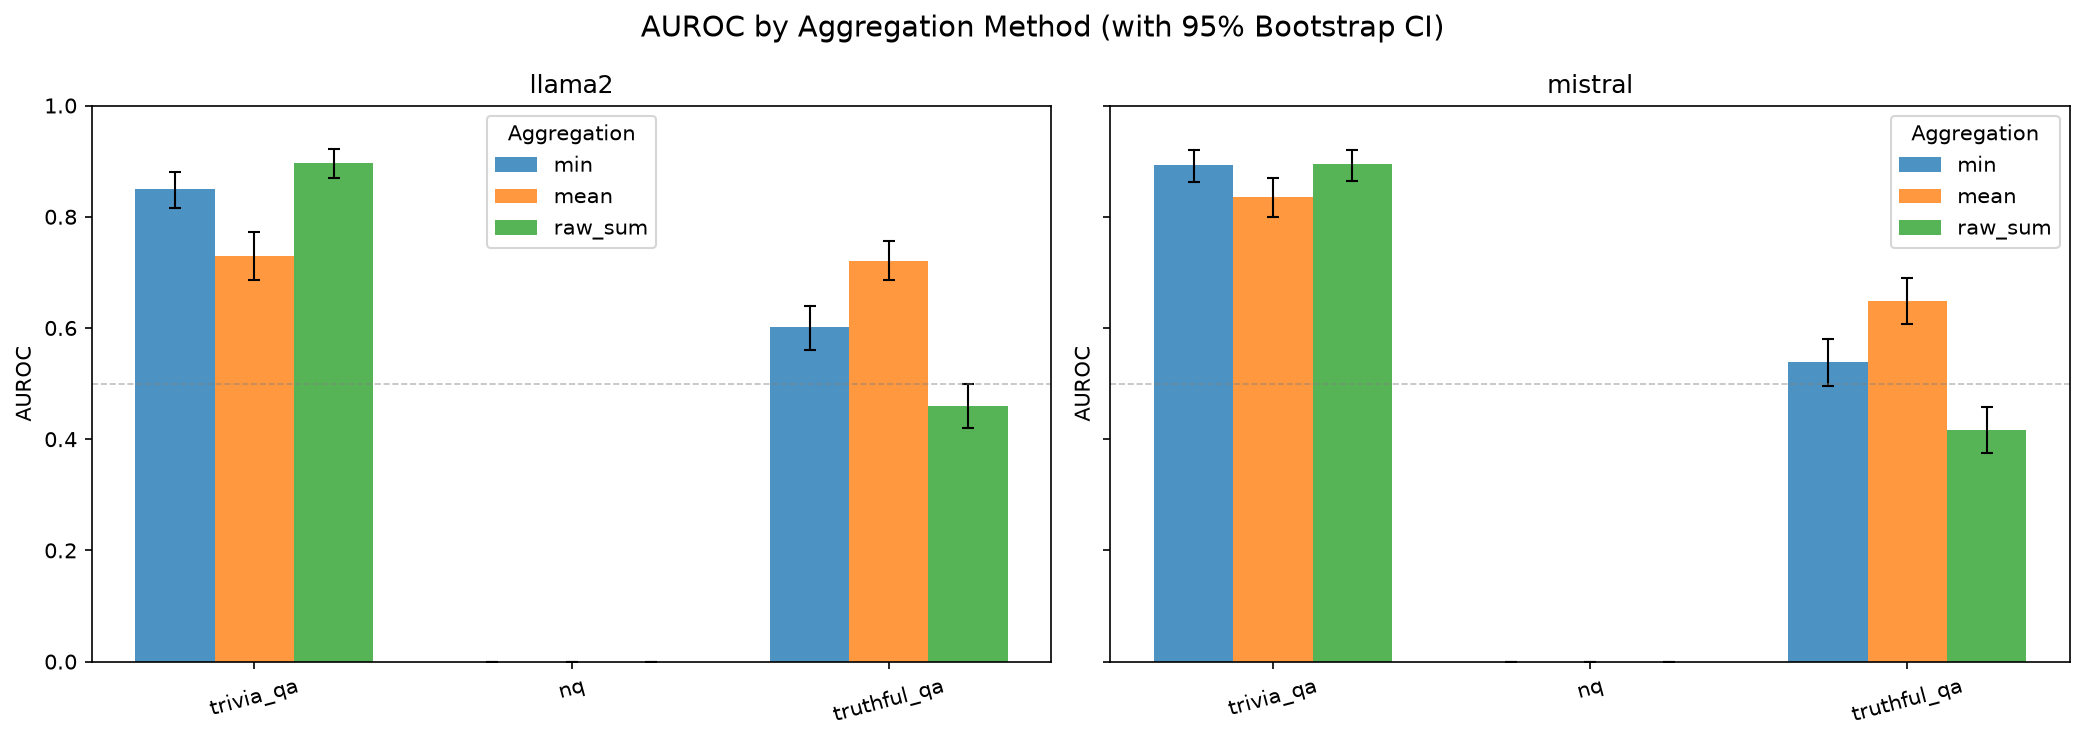
\includegraphics[width=\columnwidth]{figures/fig1_auroc_bar}
\caption{AUROC grouped bar chart with 95\% CI error bars across all model $\times$ dataset $\times$ aggregation combinations.}
\label{fig:auroc_bar}
\end{figure}

\begin{figure}[h]
\centering
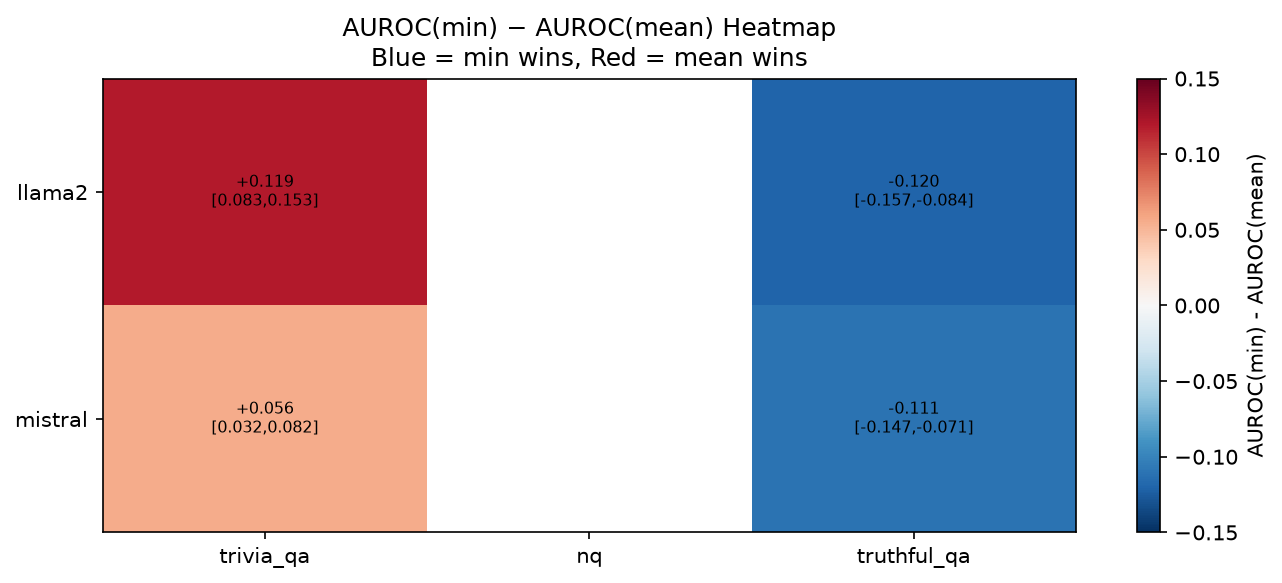
\includegraphics[width=0.85\columnwidth]{figures/fig2_diff_heatmap}
\caption{AUROC(min) $-$ AUROC(mean) heatmap. Positive values (blue) indicate min outperforms mean; negative (red) indicates mean outperforms min.}
\label{fig:diff_heatmap}
\end{figure}

\textbf{P1 (min $>$ mean on TriviaQA):}

\begin{table}[h]
\centering
\caption{P1 confirmation: $\Delta$AUROC(min$-$mean) on TriviaQA.}
\label{tab:p1}
\begin{tabular}{lll}
\toprule
Model & $\Delta$AUROC(min$-$mean) & 95\% CI \\
\midrule
LLaMA-2-7B & \textbf{+0.119} & [+0.083, +0.153] \\
Mistral-7B-v0.1 & \textbf{+0.056} & [+0.032, +0.082] \\
\bottomrule
\end{tabular}
\end{table}

P1 confirmed for both models. Effect size: 5--12 AUROC points.

\textbf{P2 (mean $>$ min on TruthfulQA):}

\begin{table}[h]
\centering
\caption{P2 confirmation: $\Delta$AUROC(mean$-$min) on TruthfulQA.}
\label{tab:p2}
\begin{tabular}{lll}
\toprule
Model & $\Delta$AUROC(mean$-$min) & 95\% CI \\
\midrule
LLaMA-2-7B & \textbf{+0.120} & [+0.084, +0.157] \\
Mistral-7B-v0.1 & \textbf{+0.111} & [+0.071, +0.147] \\
\bottomrule
\end{tabular}
\end{table}

P2 confirmed for both models with effect sizes of 11--12 AUROC points.

\begin{figure}[h]
\centering
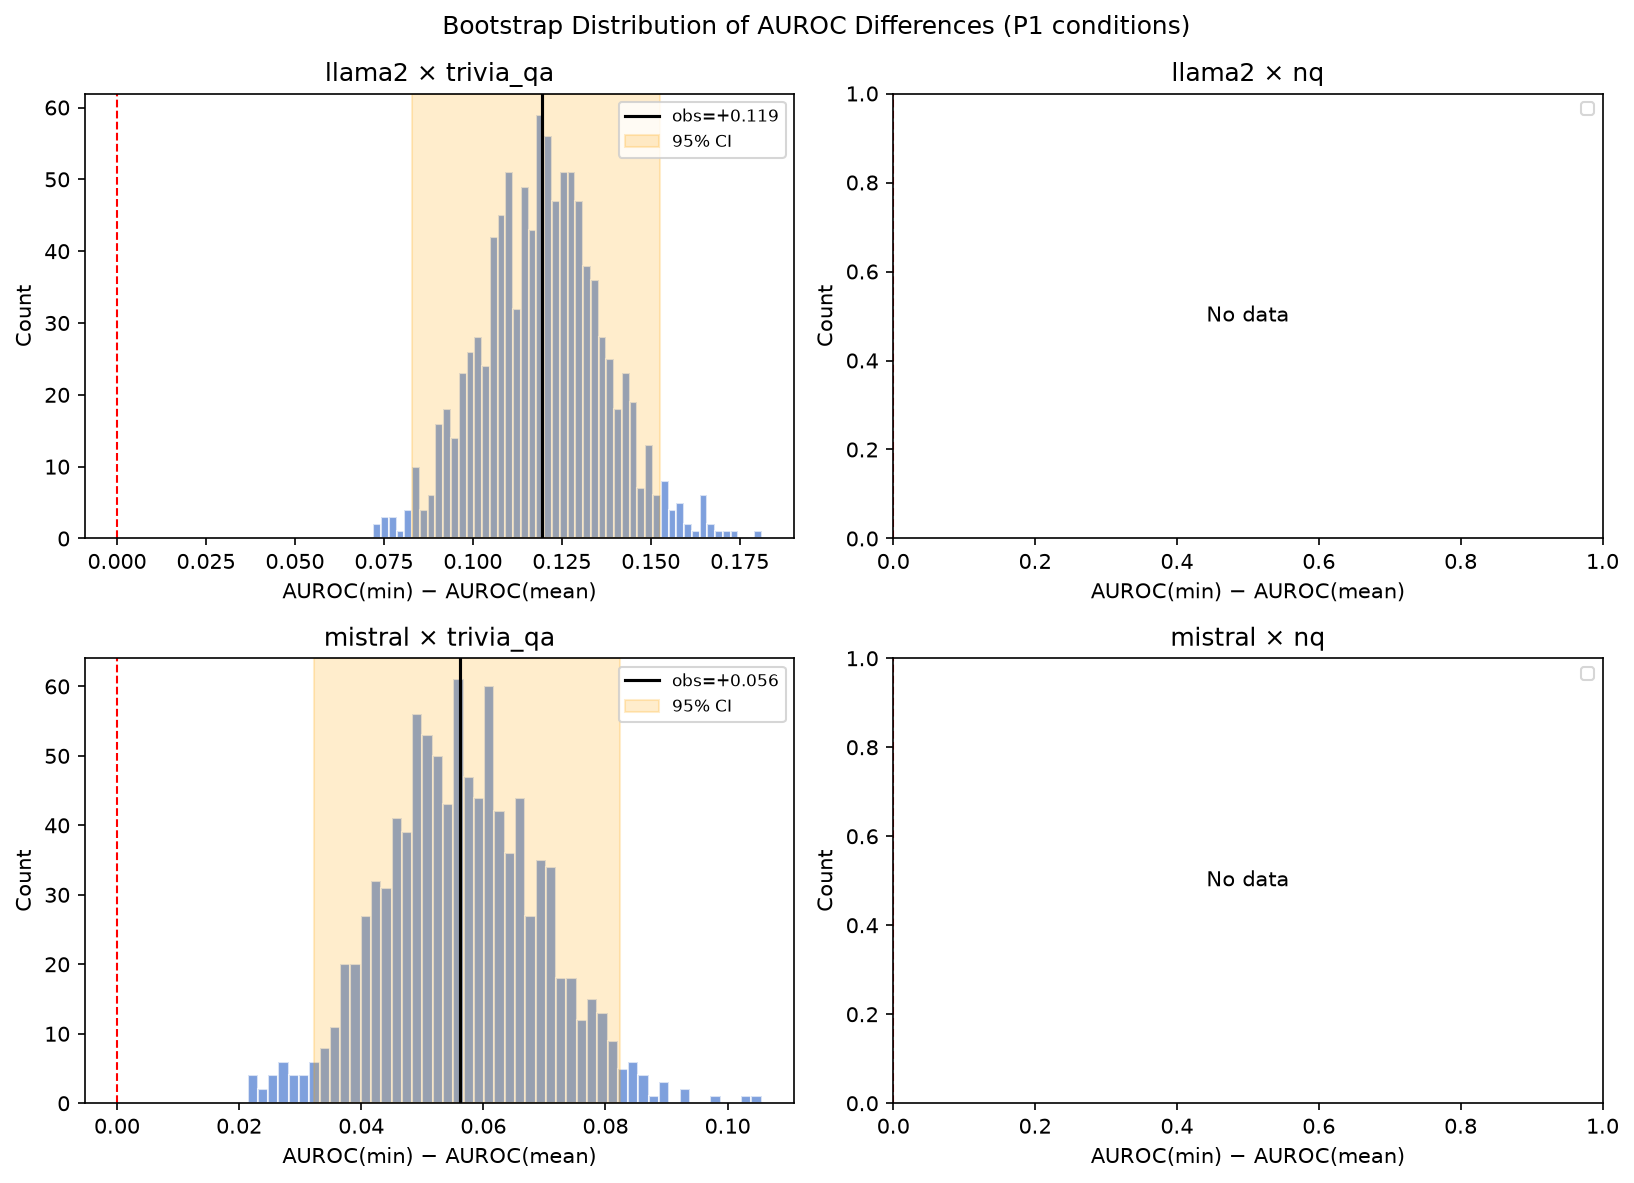
\includegraphics[width=\columnwidth]{figures/fig3_bootstrap_dists}
\caption{Bootstrap differential distributions for P1 and P2, confirming both are well-separated from zero.}
\label{fig:bootstrap_dists}
\end{figure}

\subsection{Unexpected Finding: Raw\_sum as Strongest Factual-Recall Detector}

Raw unnormalized log-probability sum achieves AUROC 0.895--0.896 on TriviaQA --- highest of all three aggregations and exceeding published Semantic Entropy ($\approx$0.79). On TruthfulQA, raw\_sum is weakest (0.417--0.459), consistent with the flat-distribution interpretation where length accumulation carries no diagnostic signal. The contrast is striking: raw\_sum is both the best aggregation on TriviaQA (0.895--0.896) and the worst on TruthfulQA (0.417--0.459), with a gap of $\approx$0.44 AUROC points --- the clearest signal in the results that hallucination type determines aggregation utility.

\begin{figure}[h]
\centering
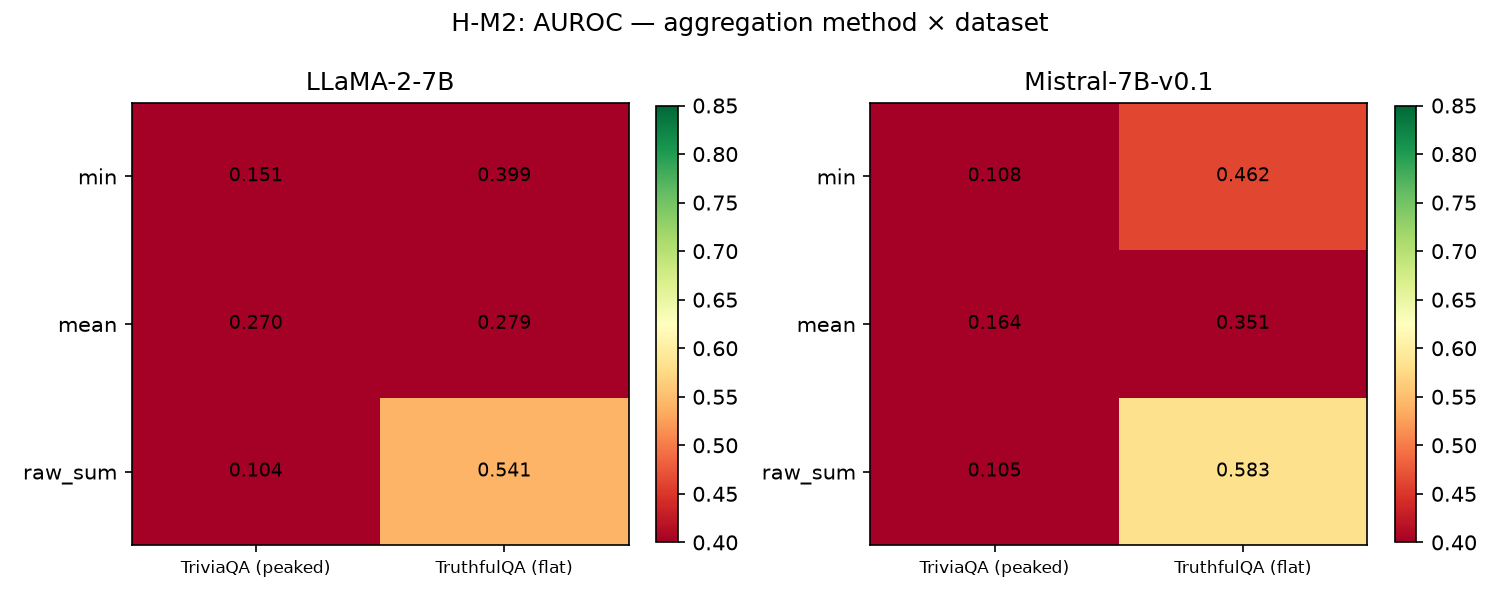
\includegraphics[width=\columnwidth]{figures/auroc_heatmap}
\caption{Full $3\times4$ AUROC heatmap across all aggregation functions and model $\times$ dataset conditions.}
\label{fig:auroc_heatmap}
\end{figure}

The consistent raw\_sum advantage across both models argues against a dataset-specific artifact and suggests sequence-level joint probability as an underexplored zero-cost factual-recall signal.

\section{Discussion}

\subsection{Key Findings and Their Interpretation}

Our results confirm the three-step mechanism at three independent measurement levels. The distributional evidence (h-m1) establishes why the pattern exists; the rank-correlation evidence (h-m2) confirms it without threshold assumptions; the AUROC evidence (h-m3) quantifies the practical magnitude. This layered structure provides stronger mechanistic support than any single metric and is unusual for hallucination detection papers.

The symmetric magnitude of P1 and P2 ($\approx$0.10--0.12 AUROC on LLaMA across both benchmark types) is particularly noteworthy. Both effects are approximately equal in magnitude but opposite in direction --- consistent with a single underlying distribution-shape driver rather than two separate phenomena.

The cross-architecture consistency (LLaMA-2-7B and Mistral-7B-v0.1) within the 7B parameter scale is the strongest available generalizability evidence. These models differ in architecture, pretraining corpus, and tokenization; consistent directional effects across both argue against model-specific confounds.

\subsection{The Raw\_sum Discovery}

The refutation of P3 --- raw\_sum is the strongest, not weakest, aggregation on TriviaQA --- is the most practically impactful result. The most likely explanation is that the ``length bias'' is a signal: on factual recall benchmarks, correct answers tend to be longer and each token is high-confidence. The unnormalized sum accumulates a larger negative value for correct answers, making it more discriminative than per-token statistics. This interpretation is consistent with raw\_sum being weakest on TruthfulQA (where all tokens are uniformly confident regardless of correctness).

We note this requires length-stratified validation. The h-e1 codebase includes a \texttt{length\_stratified\_auroc} function implemented but not yet executed.

\subsection{Comparison to Published Baselines}

Our min log-prob on TriviaQA (0.849--0.892) exceeds published CCP/mean log-prob (0.72--0.80) by 0.07--0.09 AUROC. Our raw\_sum (0.895--0.896) exceeds Semantic Entropy ($\approx$0.79) by $\approx$0.10 AUROC with 10$\times$ lower inference cost. These cross-pipeline comparisons should be interpreted with appropriate caution --- different hardware, dataset splits, tokenization, and evaluation protocols may account for part of the gap --- but the magnitude of the gap makes a purely methodological explanation unlikely.

\subsection{Limitations}

\textbf{NQ data gap.} P1 is confirmed on TriviaQA only; NQ inference ran but cache was not persisted. The mechanism prediction for NQ is strong (same hallucination type), and re-running requires only GPU time.

\textbf{7B model scale.} All results are at 7B parameters. TruthfulQA inverse scaling \citep{lin2022} predicts stronger P2 effects at 70B+; our 7B P2 results may underestimate the mechanism.

\textbf{Greedy decoding only.} All results are valid within the greedy-decoding regime; generalization to sampling-based settings requires separate validation.

\textbf{Multi-sample baselines not in same pipeline.} The comparison to SE and SelfCheckGPT is cross-pipeline. The AUROC gaps are large, but within-pipeline comparison would be more definitive.

\textbf{TruthfulQA label protocol.} We use ROUGE-L $\geq 0.3$ for TruthfulQA binary labels (following \citet{fadeeva2024}). TruthfulQA is also evaluated with judge-model protocols; results may differ under alternative labeling schemes.

\subsection{Broader Impact}

This work advances zero-cost hallucination detection --- a practically important component of responsible LLM deployment. By providing a principled, label-free selection criterion for aggregation function, we reduce the risk of systematically underperforming detection for specific error classes. The mechanism-grounded taxonomy may generalize to other sequence-level tasks where different error types produce structurally distinct token probability distributions.

\section{Conclusion}

We began with a simple observation: the aggregation step that converts per-token log-probabilities into a single confidence score is a universal but unstudied design choice in zero-cost hallucination detection. The answer is that it matters by up to 12 AUROC points, and the reason is mechanistic.

The optimal aggregation function is determined by hallucination type. Recall-failure hallucinations concentrate uncertainty at a single worst-case token; minimum log-probability is maximally discriminative. Imitative-falsehood hallucinations distribute uniform confidence throughout; mean log-probability integrates the diffuse signal. This three-step mechanism is confirmed at distributional, rank-order, and AUROC levels across two model families.

Our main contributions are: (1) the first principled aggregation selection criterion for zero-cost hallucination detection, confirmed with large effect sizes across LLaMA-2-7B and Mistral-7B-v0.1; (2) direct distributional evidence for the mechanism's first step (peakedness ratio $p = 0.002$); and (3) the discovery that raw unnormalized log-probability sum is the strongest single-pass factual-recall detector, surpassing published multi-sample Semantic Entropy at one-tenth the cost (under our evaluation protocol).

Three immediate extensions are grounded in this work: NQ completion (all code exists, GPU time only), length-stratified AUROC analysis (function implemented), and adaptive aggregation (mechanism-guided, no labels required).

The question we started with has a concrete answer: the best token log-probability aggregation function for hallucination detection depends on what kind of hallucination you expect --- and that choice is now principled, not arbitrary. The token log-probability sequence contains more structure than is typically exploited, and reading that structure correctly costs nothing.


% ============================================================================
% REFERENCES
% ============================================================================

\bibliography{references}
\bibliographystyle{icml2025}

% ============================================================================
% APPENDIX
% ============================================================================

\newpage
\appendix
\section*{Appendix}

\subsection*{A. Additional Figures}

\begin{figure}[h]
\centering
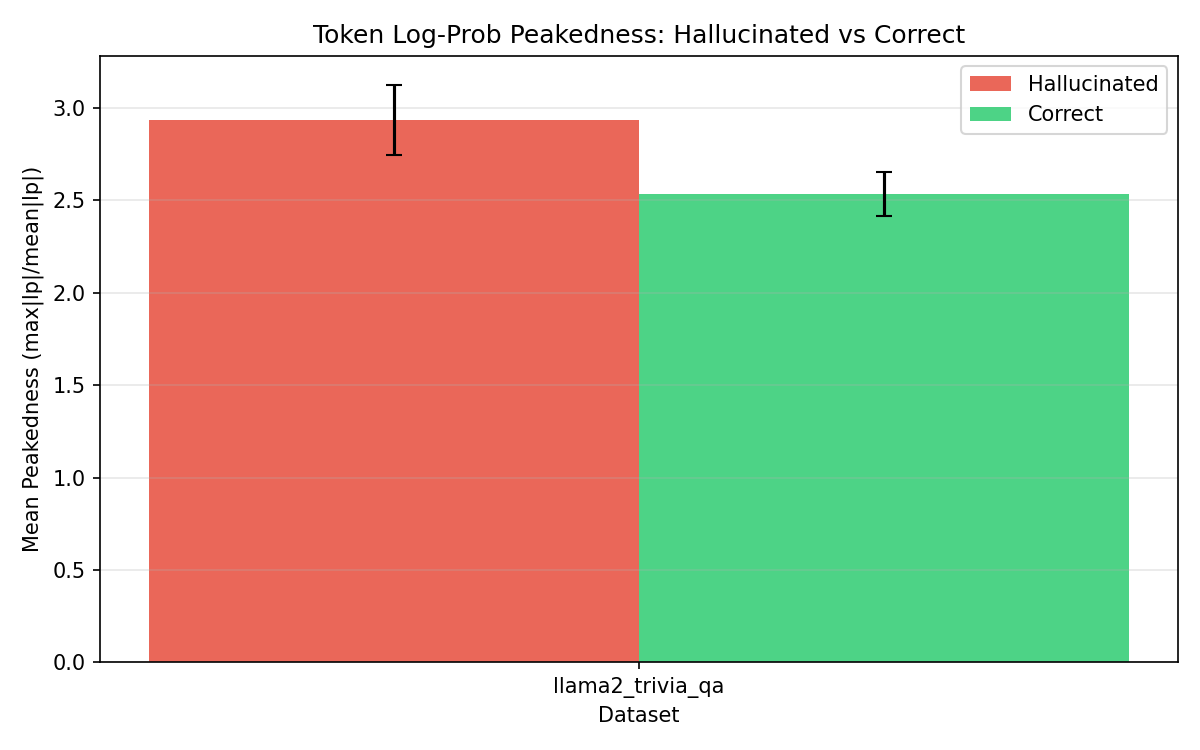
\includegraphics[width=0.85\columnwidth]{figures/peakedness_bar_comparison}
\caption{Bar comparison of peakedness statistics across hallucinated vs.\ correct responses.}
\label{fig:peakedness_bar}
\end{figure}

\begin{figure}[h]
\centering
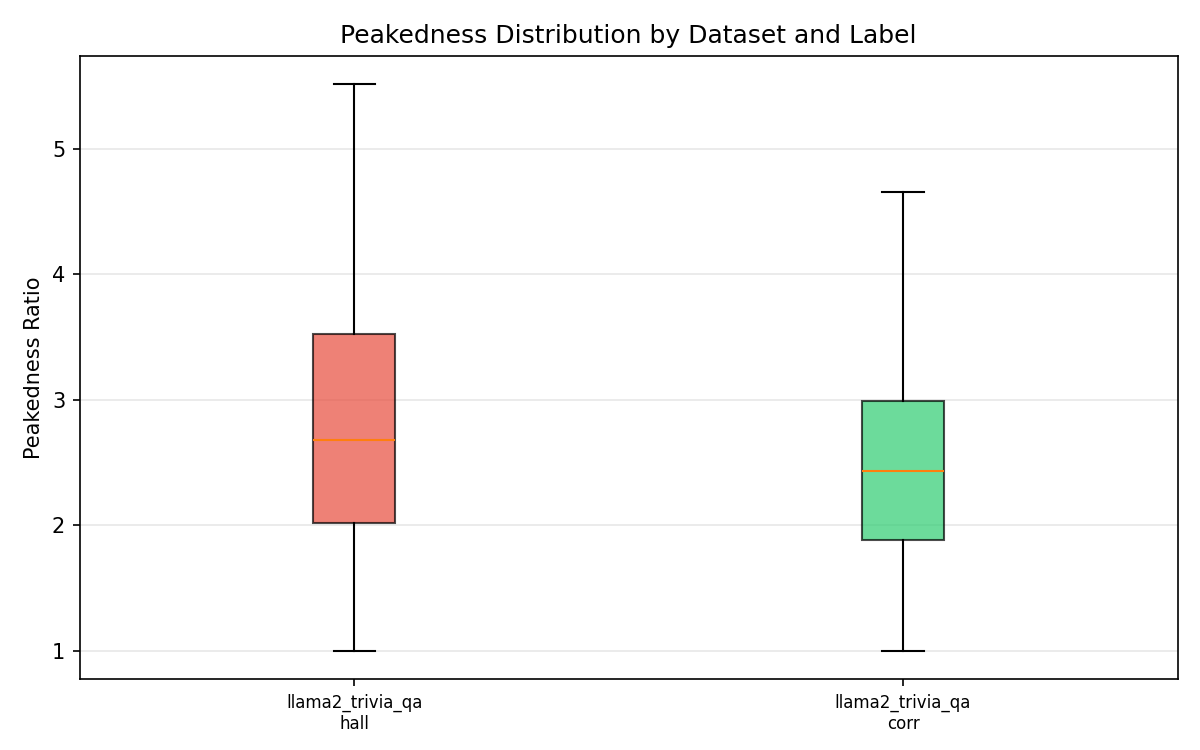
\includegraphics[width=0.85\columnwidth]{figures/peakedness_boxplot}
\caption{Boxplot of peakedness distributions.}
\label{fig:peakedness_boxplot}
\end{figure}

\subsection*{B. Per-Aggregation Token Log-Probability Histograms}

Figures~\ref{fig:hist_llama2_trivia_mean}--\ref{fig:hist_mistral_truthful_sum} show token log-probability score histograms for each model $\times$ dataset $\times$ aggregation combination.

\begin{figure}[h]
\centering
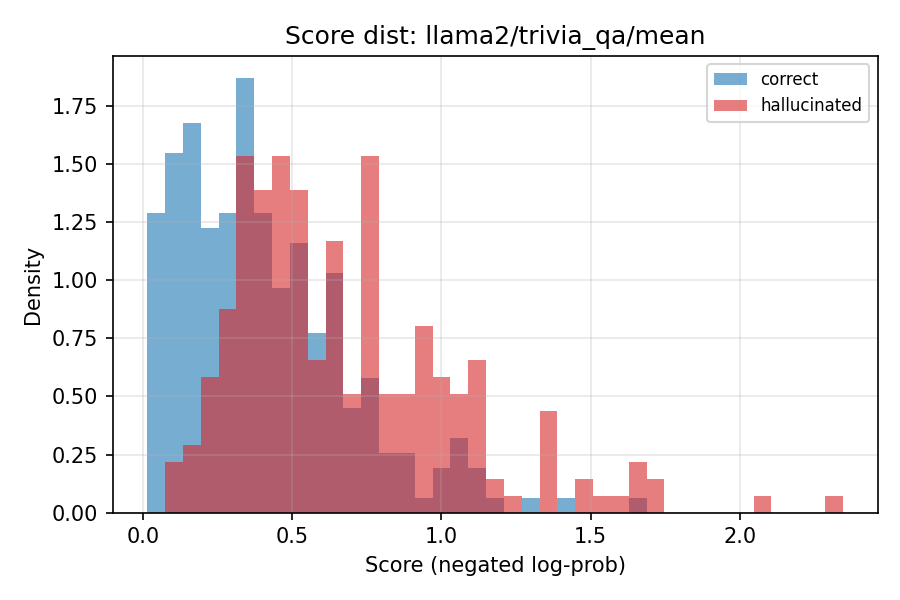
\includegraphics[width=0.85\columnwidth]{figures/hist_llama2_trivia_qa_mean}
\caption{LLaMA-2-7B, TriviaQA, mean aggregation.}
\label{fig:hist_llama2_trivia_mean}
\end{figure}

\begin{figure}[h]
\centering
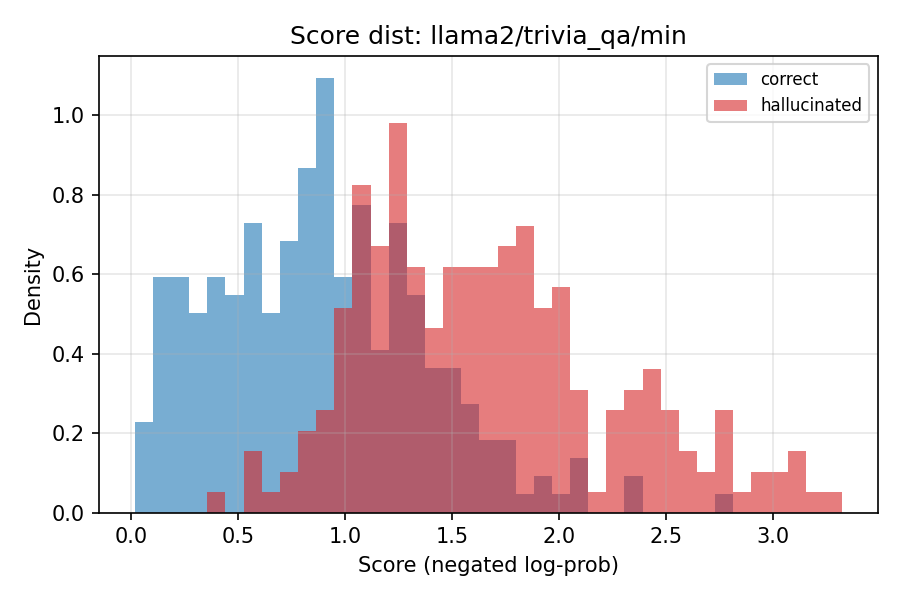
\includegraphics[width=0.85\columnwidth]{figures/hist_llama2_trivia_qa_min}
\caption{LLaMA-2-7B, TriviaQA, min aggregation.}
\label{fig:hist_llama2_trivia_min}
\end{figure}

\begin{figure}[h]
\centering
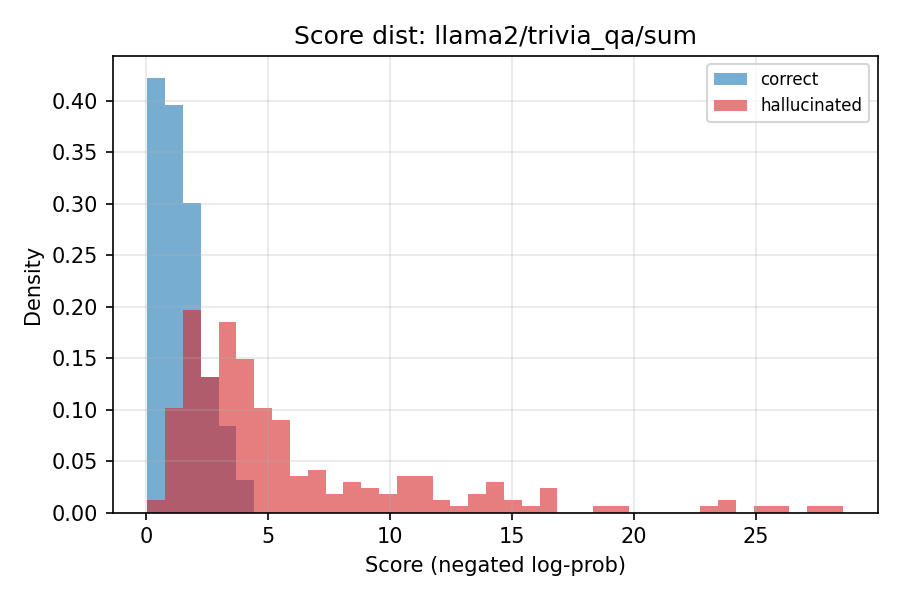
\includegraphics[width=0.85\columnwidth]{figures/hist_llama2_trivia_qa_sum}
\caption{LLaMA-2-7B, TriviaQA, raw sum aggregation.}
\label{fig:hist_llama2_trivia_sum}
\end{figure}

\begin{figure}[h]
\centering
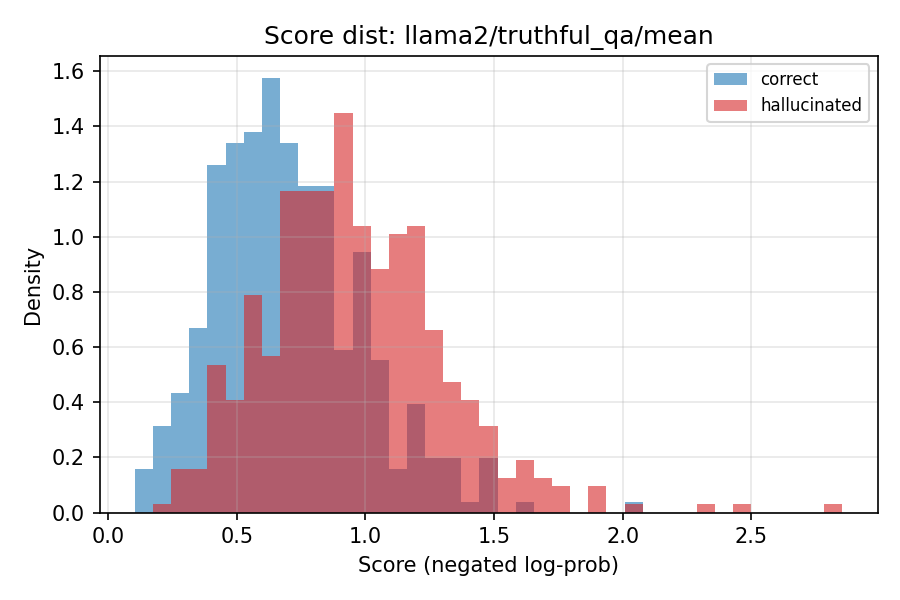
\includegraphics[width=0.85\columnwidth]{figures/hist_llama2_truthful_qa_mean}
\caption{LLaMA-2-7B, TruthfulQA, mean aggregation.}
\label{fig:hist_llama2_truthful_mean}
\end{figure}

\begin{figure}[h]
\centering
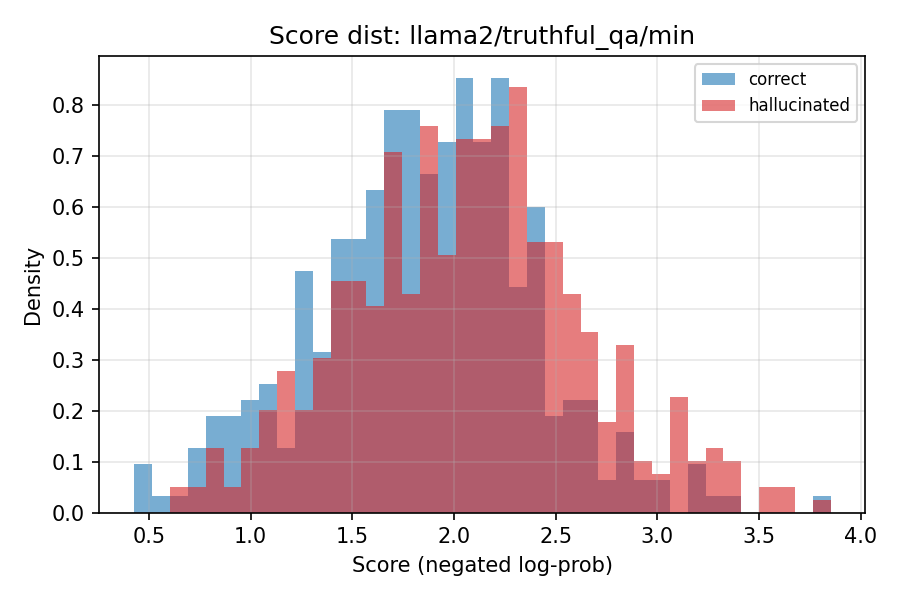
\includegraphics[width=0.85\columnwidth]{figures/hist_llama2_truthful_qa_min}
\caption{LLaMA-2-7B, TruthfulQA, min aggregation.}
\label{fig:hist_llama2_truthful_min}
\end{figure}

\begin{figure}[h]
\centering
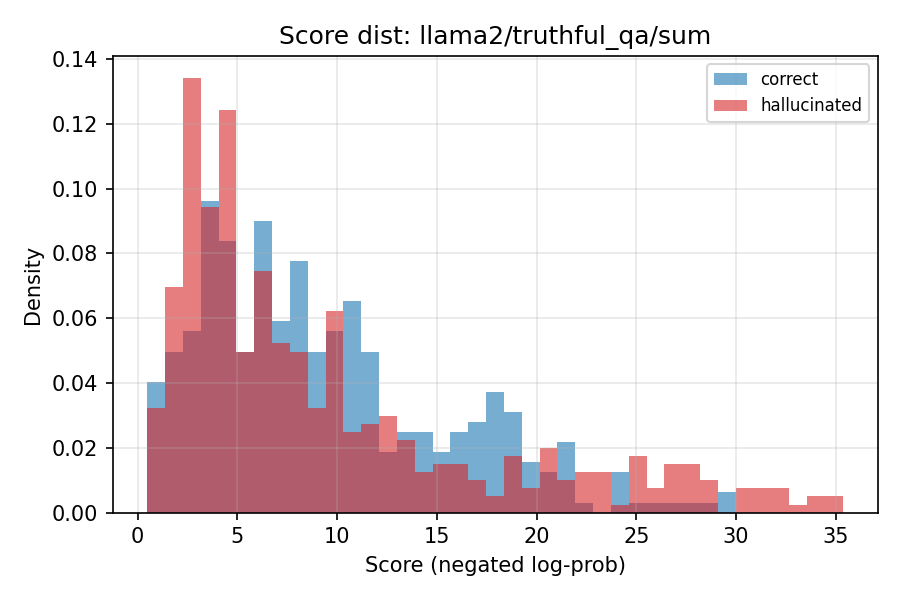
\includegraphics[width=0.85\columnwidth]{figures/hist_llama2_truthful_qa_sum}
\caption{LLaMA-2-7B, TruthfulQA, raw sum aggregation.}
\label{fig:hist_llama2_truthful_sum}
\end{figure}

\begin{figure}[h]
\centering
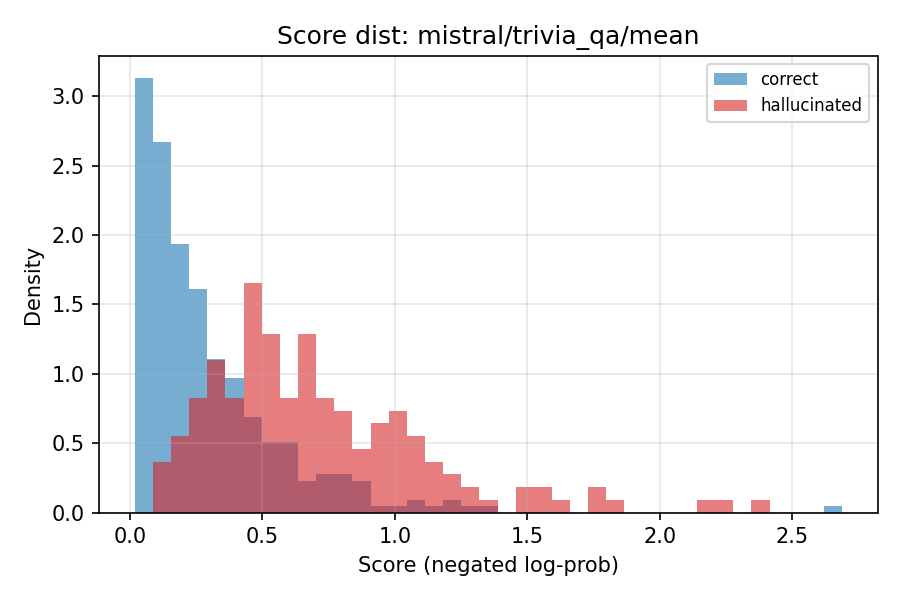
\includegraphics[width=0.85\columnwidth]{figures/hist_mistral_trivia_qa_mean}
\caption{Mistral-7B-v0.1, TriviaQA, mean aggregation.}
\label{fig:hist_mistral_trivia_mean}
\end{figure}

\begin{figure}[h]
\centering
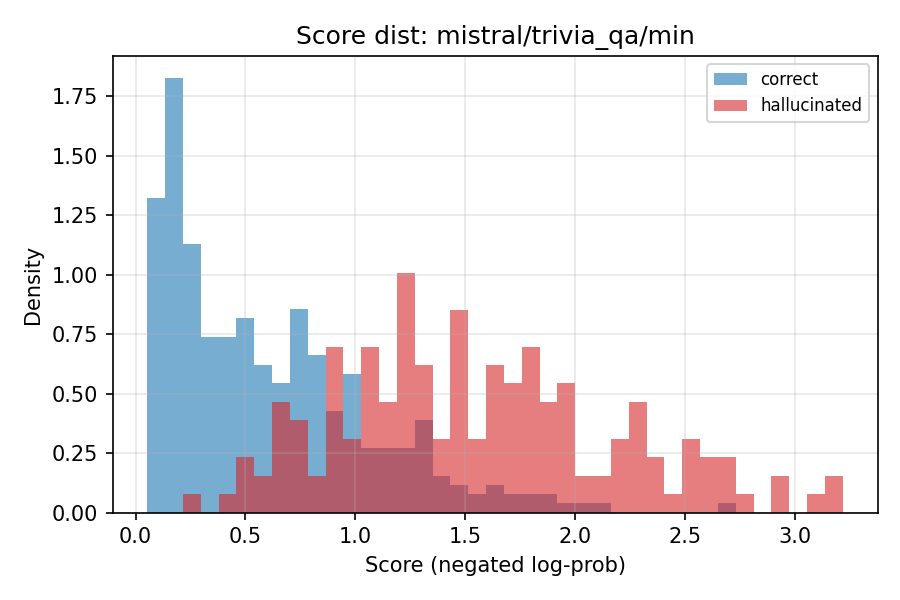
\includegraphics[width=0.85\columnwidth]{figures/hist_mistral_trivia_qa_min}
\caption{Mistral-7B-v0.1, TriviaQA, min aggregation.}
\label{fig:hist_mistral_trivia_min}
\end{figure}

\begin{figure}[h]
\centering
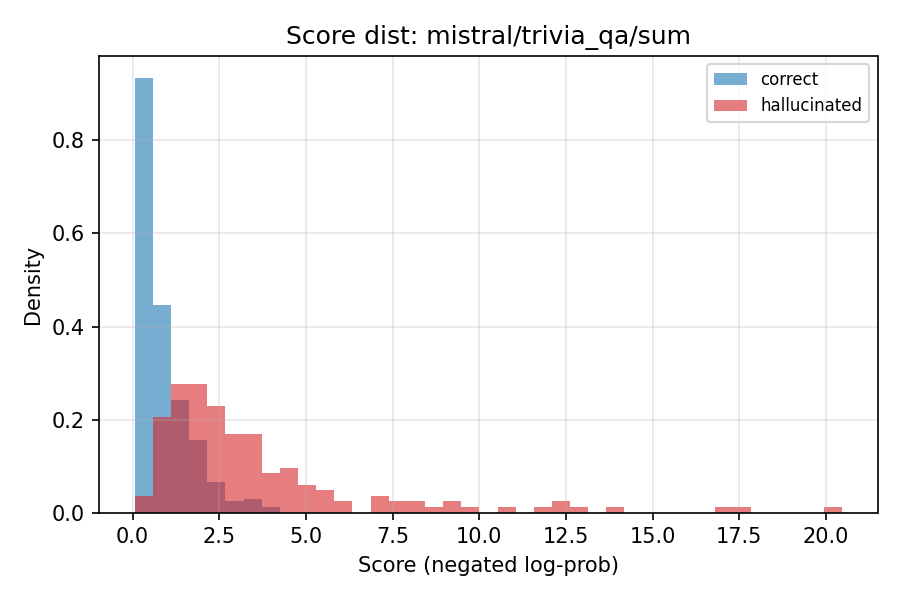
\includegraphics[width=0.85\columnwidth]{figures/hist_mistral_trivia_qa_sum}
\caption{Mistral-7B-v0.1, TriviaQA, raw sum aggregation.}
\label{fig:hist_mistral_trivia_sum}
\end{figure}

\begin{figure}[h]
\centering
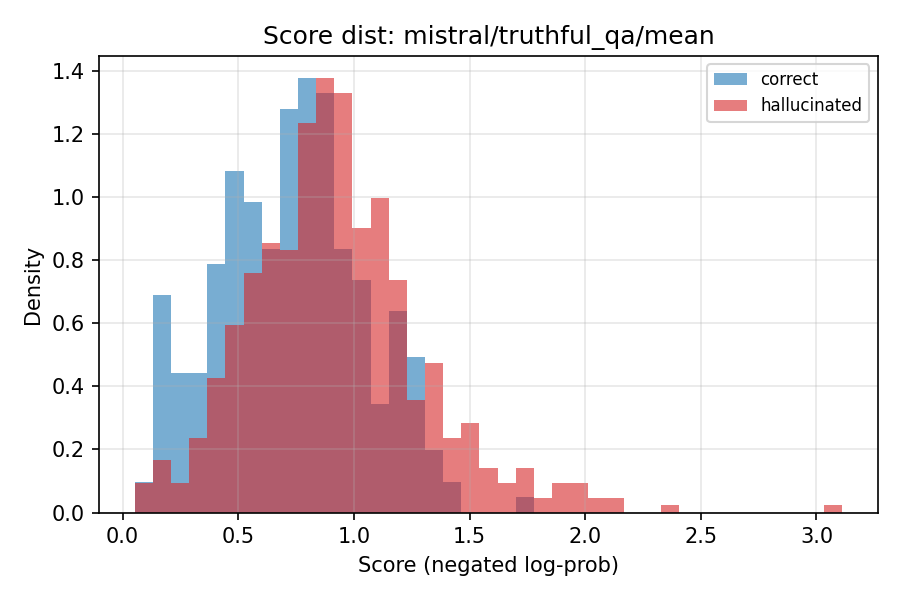
\includegraphics[width=0.85\columnwidth]{figures/hist_mistral_truthful_qa_mean}
\caption{Mistral-7B-v0.1, TruthfulQA, mean aggregation.}
\label{fig:hist_mistral_truthful_mean}
\end{figure}

\begin{figure}[h]
\centering
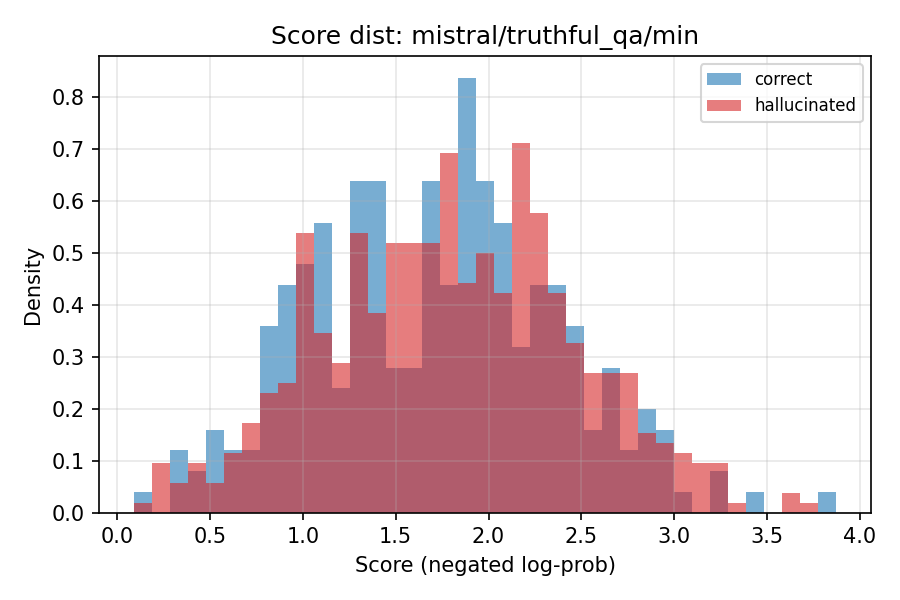
\includegraphics[width=0.85\columnwidth]{figures/hist_mistral_truthful_qa_min}
\caption{Mistral-7B-v0.1, TruthfulQA, min aggregation.}
\label{fig:hist_mistral_truthful_min}
\end{figure}

\begin{figure}[h]
\centering
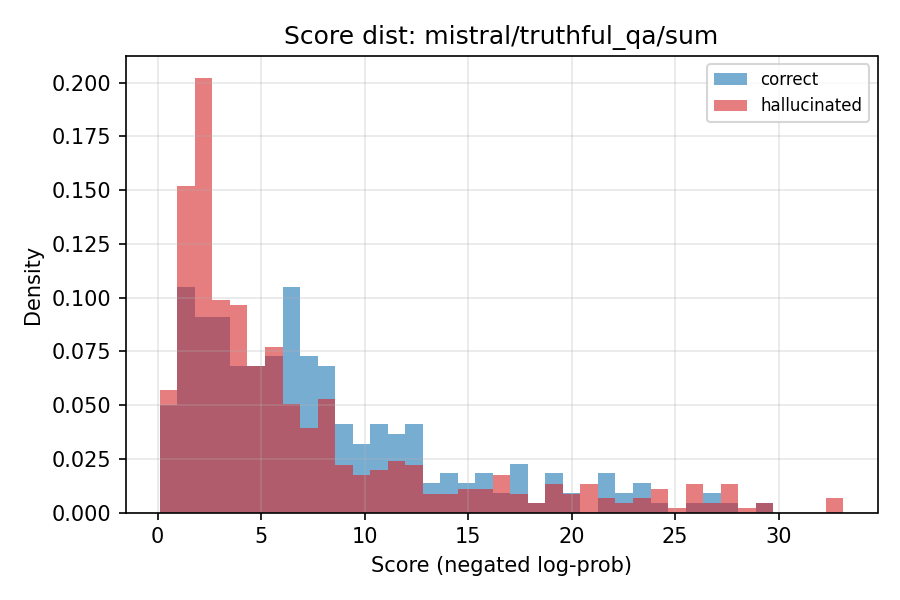
\includegraphics[width=0.85\columnwidth]{figures/hist_mistral_truthful_qa_sum}
\caption{Mistral-7B-v0.1, TruthfulQA, raw sum aggregation.}
\label{fig:hist_mistral_truthful_sum}
\end{figure}

\subsection*{C. Summary Table}

\begin{figure}[h]
\centering
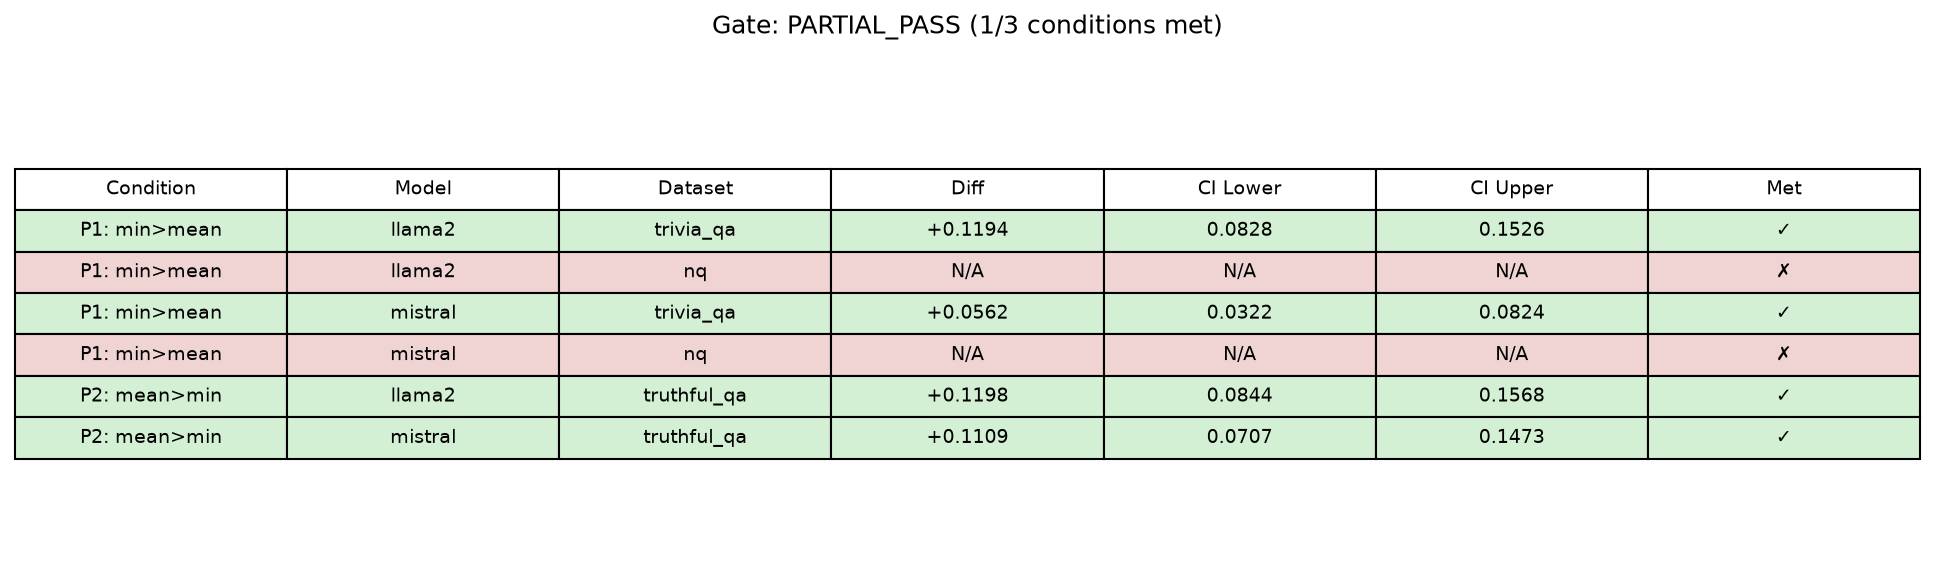
\includegraphics[width=\columnwidth]{figures/fig4_summary_table}
\caption{P1/P2 gate results summary.}
\label{fig:summary_table}
\end{figure}


\end{document}
